%%%%% TODO %%%%%

% 5. Make an inset in Figure 1 showing the NE Pacific Ocean (PNW)?
% 7. If we add JS as an author, remove Personal Communications and Acknowledgements

%%%%% Preamble %%%%%

% Set document style and font size
\documentclass[12pt]{article}

% Style file for DFO Technical Reports
\usepackage{techreport}

% New definitions: Title, year, report number, authors
% Put words in math mode to prevent case changes (e.g., species name)
\newcommand{\trTitle}{Calculating the spawn index for Pacific herring ($Clupea$ $pallasii$) in British Columbia, Canada}
\newcommand{\trYear}{2017}
\newcommand{\trReportNum}{XXXX}
\newcommand{\trAuthFootA}{\footnote{E-mail: \texttt{Matthew.Grinnell@dfo-mpo.gc.ca} $|$ telephone: (250)~756.7055}}
\newcommand{\trAuthsLong}{Matthew H.~Grinnell,\trAuthFootA{} and others...}  % JC, MT, JS...
\newcommand{\trAuthsBack}{Grinnell, M.\,H., et al...}

% New definition: Address
\newcommand{\trAddy}{Fisheries and Oceans Canada\\Science Branch, Pacific Region\\Pacific Biological Station\\3190 Hammond Bay Road\\Nanaimo, BC \enskip V9T 6N7}

% New definition: Citation
\newcommand{\trReference}{
\begin{hangparas}{1em}{1}
\trAuthsBack{} \trYear{}. \trTitle{}. Can. Tech. Rep. Fish. Aquat. Sci. \trReportNum{}: \pageref{TRlastRoman}{}\,+\,\pageref{LastPage}{}\,p.
\end{hangparas}}

% Abstract
\newcommand{\trAbstract}{
The spawn index time series is one component of Pacific herring ($Clupea$ $pallasii$) stock assessments in British Columbia (BC), Canada.
This report documents the calculations used to convert spawn survey observations (e.g., number of egg layers, extent, substrate) to the spawn index.
There are three types of spawn survey observations: surface observations, underwater observations of spawn on Macrocystis ($Macrocystis$ spp.), and underwater observations of spawn on understory.
There are several major steps to calculating the spawn index.
First, we quantify Pacific herring fecundity, which is critical to calculating the spawn index.
Second, we describe the calculations for each of the three spawn survey types: surface, Macrocystis, and understory.
Finally, we combine the three spawn indices, and aggregate by year and stock assessment region to match the temporal and spatial scale of science advice and fishery management for Pacific herring in BC.
In addition, we describe some sources of uncertainty in the spawn index calculations.
Note that the `spawn index' is not scaled by the spawn survey scaling parameter, $q$ and therefore is not an estimate of spawning stock biomass.}

% Resume (i.e., French abstract)
\newcommand{\trResume}{
[Et en fran�ais...]
}

% Set document options
%\linenumbers  % For drafts
%\onehalfspacing  % For drafts

% Let it begin
\begin{document}

% Sections in capitals
\renewcommand\listfigurename{LIST OF FIGURES}
\renewcommand\listtablename{LIST OF TABLES}

% Footnote symbols in front matter
\renewcommand*{\thefootnote}{\fnsymbol{footnote}}

%%%% Front matter %%%%%

% Format the first few pages
\thispagestyle{fancyplain}
\noindent
\begin{flushleft}
\LARGE
\textbf{\trTitle{}}
\vfill
\Large
\trAuthALong{}, and \trAuthBLong{}
\vfill
\trAddy{}
\vfill
\trYear{}
\vfill
\LARGE
\textbf{Canadian Technical Report of\\
Fisheries and Aquatic Sciences \trReportNum{}}
\lfoot{
\includegraphics[height=7mm]{Document/LogoDFO.png}}
\cfoot{}
\rfoot{
\includegraphics[height=7mm]{Document/LogoCanada.jpg}}
\end{flushleft}
\clearpage
  % Cover page
\footnotesize
\lfoot{} \cfoot{\thepage} \rfoot{}
\thispagestyle{empty}
\begin{center}
\textbf{Canadian Technical Report of Fisheries and Aquatic Sciences}
\end{center}
\noindent
Technical reports contain scientific and technical information that contributes to existing knowledge but which is not normally appropriate for primary literature.
Technical reports are directed primarily toward a worldwide audience and have an international distribution.
No restriction is placed on subject matter and the series reflects the broad interests and policies of Fisheries and Oceans Canada, namely, fisheries and aquatic sciences.
\indent
\par
Technical reports may be cited as full publications.
The correct citation appears above the abstract of each report.
Each report is abstracted in the data base \emph{Aquatic Sciences and Fisheries Abstracts}.
\par
Technical reports are produced regionally but are numbered nationally.
Requests for individual reports will be filled by the issuing establishment listed on the front cover and title page.
Out-of-stock reports will be supplied for a fee by commercial agents.
\par
Numbers 1--456 in this series were issued as Technical Reports of the Fisheries Research Board of Canada.
Numbers 457--714 were issued as Department of the Environment, Fisheries and Marine Service, Research and Development Directorate Technical Reports.
Numbers 715--924 were issued as Department of Fisheries and Environment, Fisheries and Marine Service Technical Reports.
The current series name was changed with report number 925.
\bigskip
\begin{center}
\textbf{Rapport technique canadien des sciences halieutiques et aquatiques}
\end{center}
\noindent
Les rapports techniques contiennent des renseignements scientifiques et techniques qui constituent une contribution aux connaissances actuelles, mais qui ne sont pas normalement appropri�s pour la publication dans un journal scientifique.
Les rapports techniques sont destin�s essentiellement � un public international et ils sont distribu�s � cet �chelon.
II n'y a aucune restriction quant au sujet; de fait, la s�rie refl�te la vaste gamme des int�r�ts et des politiques de P�ches et Oc�ans Canada, c'est-�-dire les sciences halieutiques et aquatiques.
\indent
\par
Les rapports techniques peuvent �tre cit�s comme des publications � part enti�re.
Le titre exact figure au-dessus du r�sum� de chaque rapport.
Les rapports techniques sont r�sum�s dans la base de donn�es \emph{R�sum�s des sciences aquatiques et halieutiques}.
\par
Les rapports techniques sont produits � l'�chelon r�gional, mais num�rot�s � l'�chelon national.
Les demandes de rapports seront satisfaites par l'�tablissement auteur dont le nom figure sur la couverture et la page du titre.
Les rapports �puis�s seront fournis contre r�tribution par les agents commerciaux.
\par
Les num�ros 1 � 456 de cette s�rie ont �t� publi�s � titre de Rapports techniques de l'Office des recherches sur les p�cheries du Canada.
Les num�ros 457 � 714 sont parus � titre de Rapports techniques de la Direction g�n�rale de la recherche et du d�veloppement, Service des p�ches et de la mer, minist�re de l'Environnement.
Les num�ros 715 � 924 ont �t� publi�s � titre de Rapports techniques du Service des p�ches et de la mer, minist�re des P�ches et de l'Environnement.
Le nom actuel de la s�rie a �t� �tabli lors de la parution du num�ro 925.
\clearpage
  % Tech report page
\normalsize
\pagenumbering{roman}
\thispagestyle{empty}
\noindent
\begin{center}
Canadian Technical Report of\\
Fisheries and Aquatic Sciences \trReportNum{}
\vfill
\trYear{}
\vfill
\MakeTextUppercase{\trTitle{}}
\vfill
by
\vfill
\trAuthALong{},\footnote{E-mail: \trAuthAEmail{} $|$ telephone: \trAuthAPhone{}} and \trAuthBLong{}\footnote{E-mail: \trAuthBEmail{} $|$ telephone: \trAuthBPhone{}}
\vfill
\trAddy{}
\end{center}
\clearpage
  % Inside cover page
\vspace*{\fill}
\begin{center}
\begin{minipage}{\widthof{\copyright{} Her Majesty the Queen in Right of Canada, \trYear{}}}
\copyright{} Her Majesty the Queen in Right of Canada, \trYear{}\\
Cat. No. Fs97-6/\trReportNum{} E \hfill ISSN 0706-6457\\
Cat. No. Fs97-6/\trReportNum{} E-PDF \hfill ISSN 1488-5379
\end{minipage}
\end{center}
\par
\bigskip
\noindent
Correct citation for this publication:
\bigskip
\par
\begin{hangparas}{1em}{1}
\trReference{}
\end{hangparas}
\clearpage
  % Colophon page
\pdfbookmark[1]{\contentsname}{toc}  % Add TOC to pdf bookmarks (clickable)
\tableofcontents\clearpage  % Table of contents page
\listoffigures \listoftables \clearpage  % Lists of figures and tables (optional)
\noindent
\section*{ABSTRACT}
\addcontentsline{toc}{section}{ABSTRACT}
\trReference{}
\bigskip
This report documents the calculations used to convert spawn survey observations (e.g., number of egg layers, extent of spawn) to the spawn index for Pacific herring ($Clupea$ $pallasii$) in British Columbia (BC), Canada.
There are three types of spawn survey observations: surface observations, underwater observations of spawn on Macrocystis, and underwater observations of spawn on understory.
Data from these three survey types are combined to develop an overall annual spawn index for each stock assessment region in BC.
The spawn index is one component of Pacific herring stock assessments in BC.
Note that the 'spawn index' is not scaled by the spawn survey scaling parameter, $q$ and therefore is not an estimate of spawning stock biomass.
\section*{R\'{E}SUM\'{E}}
\addcontentsline{toc}{section}{R\'{E}SUM\'{E}}
\trReference{}
\bigskip
Ceci est la r�sum�...
\vfill
\label{TRlastRoman}
\clearpage
  % Abstact and resume page

% Settings for the main document
\pagenumbering{arabic}  % Regular page numbers
%\thispagestyle{empty}  % No page number on first page
\renewcommand*{\thefootnote}{\arabic{footnote}}  % Back to numeric footnotes
\setcounter{footnote}{0}  % And start at 1

% Settings for drafts
\renewcommand{\headrulewidth}{1pt}  % Header line
\pagestyle{fancy}\fancyhead[c]{Draft: Do not cite or circulate}  % Header text

%%%%% Main document %%%%%

\section{INTRODUCTION}

The spawn index time series is one component of Pacific herring ($Clupea$ $pallasii$) stock assessments in British Columbia (BC), Canada \citeyearpar[CSAS][]{CSAS2015b}.
Along with catch and biological time series, the spawn index is used to fit an integrated statistical catch-at-age model.
Key results from the stock assessment model include stock reconstructions, estimated current stock status, and projected spawning biomass in the upcoming year.
Projected spawning biomass is used to set allowable harvest levels.
Note that the `spawn index' is not scaled by the spawn survey scaling parameter, $q$ \citeyearpar[CSAS][]{CSAS2015b} and therefore is not an estimate of spawning stock biomass.

This report documents the calculations used to convert spawn survey observations (e.g., number of egg layers, extent, substrate) to the spawn index for Pacific herring in BC.
The process and calculations described in this report have been documented elsewhere, in either published or informal, internal documents.
Our goal is to collect and simplify the details necessary to understand the process for calculating the spawn index.
Spawn index calculations have been updated over the years as more data and analyses justify improvements; we restrict this report to describing the current methods.%
\footnote{Include (or mention) `old' ways of calculating egg density? 
For example, there are (at least) two ways for \autoref{eqEggDensUnderA}.
I suspect this isn't necessary/relevant, and would open up a lot of discussion: there are a lot of `old' ways to calculate the spawn index...}

The motivation to document the spawn index calculations occurred when we translated the process from a \textbf{Microsoft Access} database to an \textbf{R} \citeyearpar[RCT][]{R-3.3.2} script.
We updated from a database to an \textbf{R} script for several reasons.
First, the database has been used for various purposes over several decades, and has incidental calculations that make it overly complex.
Second, the database is difficult to troubleshoot, and to differentiate between input (i.e., data) and derived values.
Third, the \textbf{R} script is open and transparent; users are welcome to view and download the script and example data (\autoref{secDown}).
Fourth, we consider it good practice to separate data from analyses.
Finally, a separate \textbf{R} script will allow us to generate dynamic documents in the spirit of reproducible research using \textbf{knitr} \citep{Xie2015}.

Spawn surveys collect data used to calculate the spawn index.
There are three types of spawn survey observations: surface observations, underwater observations of spawn on Macrocystis ($Macrocystis$ spp.), and underwater observations of spawn on understory.
Note that understory observations have two components: spawn on substrate, and spawn on algae.
Surface spawn surveys are the least accurate of the three survey types, but they have the greatest temporal and spatial extent \citep{Schweigert1993b}.
For example, surface spawn surveys were the only survey type prior to 1988, and they are still used extensively for minor spawns, remote spawns (i.e., outside stock assessment regions; see below), and unusually early or late spawns.
Macrocystis and understory spawn surveys are conducted using SCUBA gear; underwater SCUBA surveys have been used for all major spawns since 1988.
Herring spawn surveys began in 1928, but are considered incomplete prior to 1937 because many potential areas were not surveyed (Ref?).

Herring spawn survey observations have a nested hierarchical structure: quadrats are nested within transects, transects are nested within spawns, and spawns are nested within locations.
For stock assessment purposes, locations are nested within sections, sections are nested within statistical areas, and statistical areas are nested within five major and two minor stock assessment regions (SARs) in BC.
The major SARs are Haida Gwaii, Prince Rupert District, Central Coast, Strait of Georgia, and West Coast Vancouver Island; the minor SARs are Area 27, and Area 2 West (\autoref{figBC}).
Another level of data structure is `beds', which are habitat features as opposed to distinct spatial areas.
Bed widths are used to calculate the spawn index for surface surveys.

\begin{figure}
\centering
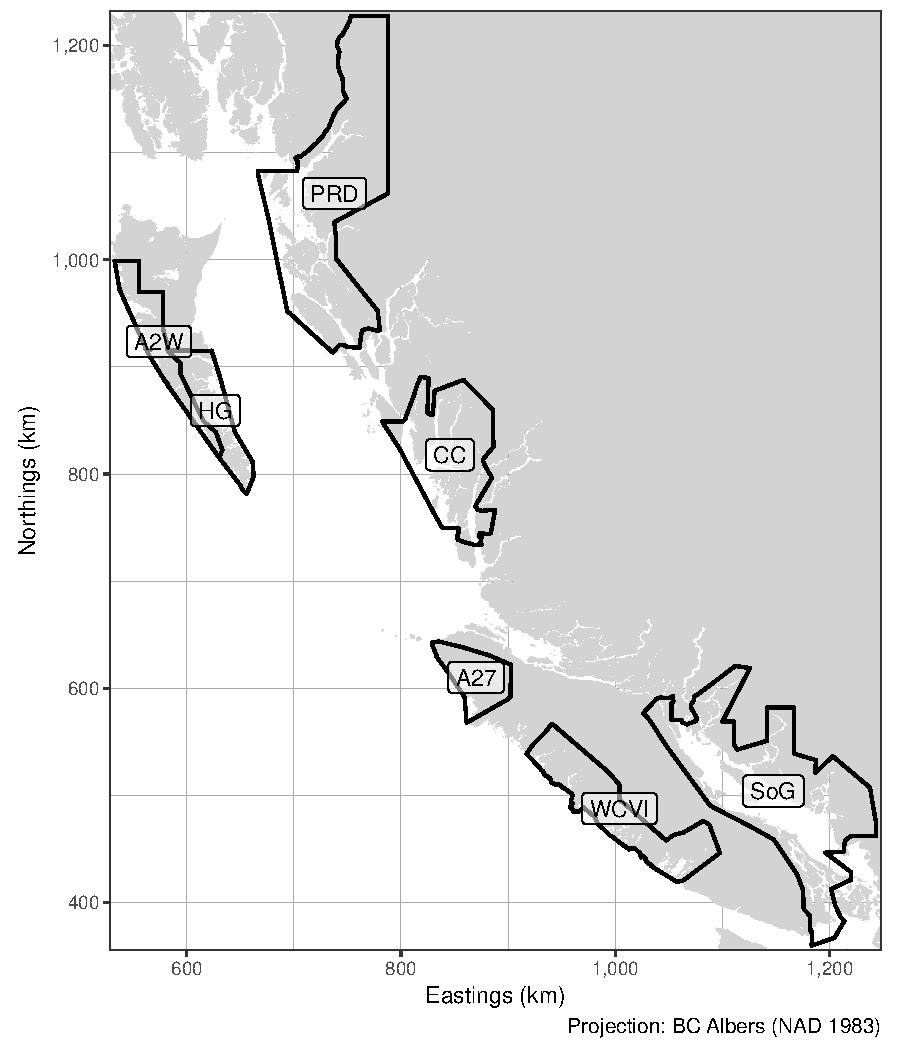
\includegraphics[width=\linewidth]{Figures/BC.pdf}
\caption[Boundaries for Pacific herring stock assessment regions (SARs)]
{Boundaries for British Columbia Pacific herring stock assessment regions (SARs): there are five major SARs (Haida Gwaii, HG; Prince Rupert District, PRD; Central Coast, CC; Strait of Georgia, SoG; and West Coast Vancouver Island, WCVI), and two minor SARs (Area 27, A27; and Area 2 West, A2W).}
\label{figBC}
\end{figure}

We have divided this report into sections for different topics.
First, we describe the data pre-processing that occurs when raw survey observations are imported into the database (\autoref{secData}).
Second, we quantify Pacific herring fecundity (\autoref{secFecund}), which is critical to calculating the spawn index.
Third, we describe the calculations for each of the three aforementioned spawn survey types: surface (\autoref{secSurf}), Macrocystis (\autoref{secMacro}), and understory (\autoref{secUnder}).
Within each section, each level of spatial aggregation (e.g., calculations at the quadrat, or transect level) is in a separate subsection.
Fourth, we combine the three spawn indices to get the total spawn index (\autoref{secTotal}).
Next, we discuss some sources of uncertainty in spawn index calculations (\autoref{secUncertain}).
Finally, we describe how users can download and run the \textbf{R} script to calculate the spawn index (\autoref{secDown}).
Note that we have avoided subscript notation in the following equations to correspond with the \textbf{R} script which does not use subscripts (e.g., no `for' loops or indexing).%make this report more accessible, and to
\footnote{We could add subscript notation if required.}

\section{DATA PRE-PROCESSING}\label{secData}

TODO:
\begin{itemize}
\item Describe the database calculations/pre-processing (if any?) that occurs in the \textbf{Microsoft Access} database when raw survey data are entered, which create the tables imported by \texttt{SpawnIndex.R} (e.g., \texttt{tSSAllspawn}, \texttt{tSSMacTrans}).
\item Reproduce these in \textbf{R} to fully understand them, instead of relying on the database?
\item (MT) Would have to look into this more, but I do not think there are any pre-calculations from the survey data entry program.
\end{itemize}

\section{SAMPLING PROTOCOL}\label{secSamp}

The following is a brief summary of the spawn survey sampling protocol in .. (Ref?).
Generally, Pacific herring spawn on substrate and algae in the intertidal and subtidal zones, to $20\,\text{m}$ deep?
We identify distinct spawns (either spatially or temporally) by a unique `spawn number.'
The spawn number is the finest scale at which we calculate the spawn index.

Herring spawns typically extend along the shore; from above spawns typically appear to be bands running parallel to the shore.
Thus, spawn `length' usually refers to distances parallel to the shore, and `width' usually refers to distances perpendicular to the shore.
For example, Macrocystis length, $LengthMacroT$ and algae length, $LengthAlgS$ refer to the distance that Macrocystis and algae extend parallel to the shore, respectively.
One exception is transect width, $TransectWidth = 2\,\text{m}$, which refers to the distance parallel to the shore.

When surveying spawn, the first task is to map out the spatial extent of the herring spawn in terms of length and width.
Next, transects are generally set $200\,\text{m}$ in from the edges, and spaced $350\,\text{m}$ apart along the length.
Transects are set perpendicular to the shore, and go from 0 to $20\,\text{m}$ depth?
Most areas where herring spawn have permanent transects which allow survey crews to replicate transects from previous years.
When permanent transects are unavailable, survey crews set new transects based on pre-specified criteria.
We then digitize these new transects to make then available as permanent transects for future spawn surveys.

\subsection{SURFACE SPAWN}

How are surface surveys conducted?

\subsection{MACROCYSTIS SPAWN}

Macrocystis spawn surveys are a census of Macrocystis plants within $1\,\text{m}$ of the transect line.
Divers categorize Macrocystis plants as either `mature' or `immature' based on stipe height.
Mature plants have stipes $\geq1\,\text{m}$ high, and are the only plants used for Macrocystis spawn index calculations.
For each mature plant, divers record the height, number of egg layers, and number of fronds.

\subsection{UNDERSTORY SPAWN}

Quardats are placed along transects, with a target of $\geq 5$ quadrats per transect, with a minimum spacing of $2\,\text{m}$, and a maximum spacing of $40\,\text{m}$.
Quadrat size for understory spawn surveys is usually $0.5\,\text{m}^{2}$; other sizes have been used for research, but not for spawn surveys.
Within each quadrat, divers record the dominant or most heavily spawned substrate type, percentage of the quadrat covered in spawn, and number of egg layers.
In addition, divers identify (at most) three dominant algae types that have spawn.
For each of these algae types, divers record the percentage of the quadrat covered by the algae, and number of egg layers.

\section{FECUNDITY}\label{secFecund}

Female Pacific herring produce an average of approximately 200 eggs per gram, g of total body weight \citep{Hay1985, HayBrett1988}.
We assume that females account for 50\% of spawners, and we use the following fecundity conversion factor for eggs to tonnes, t of spawners
\begin{equation}
\frac {1 \cdot 10^{8}~\text{eggs}} {\text{t}} = \frac{200~\text{eggs}} {\text{g}} \times 0.5 \times \frac{1 \cdot 10^{6}~\text{g}} {\text{t}} \enspace .
\label{eqFecundityConv}
\end{equation}
Note that our unit of measurement for eggs is thousands (i.e., $\text{eggs} \cdot 10^{3}$) in the \textbf{R} script, and correspondingly in this report.
Therefore, we divide $\text{eggs} \cdot 10^{3}$ by $1 \cdot 10^{5}$ to calculate an index of spawning biomass (i.e., the spawn index) in tonnes.
Although Pacific herring fecundity is affected by environmental variability and other factors, we expect that bias to the spawn index from using \autoref{eqFecundityConv} is insignificant in most areas and years \citep{Schweigert1993b}.

\section{SURFACE SPAWN}\label{secSurf}

Surface spawn surveys collect data along transects, and we calculate spawn metrics at the transect, and spawn/bed level.

\subsection{TRANSECT LEVEL CALCULATIONS}

For each substrate type, egg layers is
\begin{equation}
EggLyrs = Layers \times Proportion
\label{eqEggLayersSurf}
\end{equation}
where $Layers$ is the number of egg layers on a given substrate type, and $Proportion$ is the proportion of the transect covered by the substrate type.
At the transect level, the sum of $EggLyrs$ is $EggLyrsTotT$.
That is to say, $EggLyrsTotT$ is the sum of $EggLyrs$ for all the substrate types within a given transect.
For the time period when spawn `intensity' categories were recorded instead of estimating the number of egg layers, intensity is converted to $EggLyrsTotT$ (\autoref{tabIntensity}).
Surface egg density in thousands is \citep{SchweigertEtal1997}%
\footnote{Notwithstanding the units provided in \cite{SchweigertEtal1997}, surface egg density is in thousands ($\text{eggs} \cdot 10^{3} \cdot \text{m}^{-2}$; J.~Schweigert, personal communication, 24 February 2017).}
\begin{equation}
EggDensT = EggLyrsTotT \times 212.218 + 14.698
\label{eqEggDensSurf}
\end{equation}
where $EggDensT$ is in $\text{Eggs} \cdot 10^{3} \cdot \text{m}^{-2}$. 

\begin{table}
\centering
\caption[Spawn intensity categories and associated egg layers for Pacific herring surface spawn surveys]
{Spawn intensity categories and associated egg layers for Pacific herring surface spawn surveys for the periods 1928--1950, and 1951--1978 \citep{HumphreysHaegele1976, HayKronlund1987}.
\textbf{These values aren't directly from \citet{HumphreysHaegele1976} or \citet{HayKronlund1987}. Any idea where they're from?
Also, \citet{HayKronlund1987} says that the change from 5 to 9 categories happened in 1969, which seems to be incorrect based on intensity values in the database, unless the database was retroactively updated at some point?
They say the change from 5 to 9 categories was ``probably to accomodate the practice of reporting intermediate categories (such as 3.5).''}
Starting in 1979, spawn surveyors estimated the number of egg layers, and they continued to record intensity until 1981 to provide overlap between the two methods.
Note that intensity was sometimes recorded after being officially discontinued in 1981.
}
\begin{tabular}{ccr}
\toprule
\multicolumn{2}{c}{Intensity category} & \\
1928--1950 & 1951--1978 & Egg layers\\
\midrule
1 & 1 & 0.5529 \\
  & 2 & 0.9444 \\
2 & 3 & 1.3360 \\
  & 4 & 2.1496 \\
3 & 5 & 2.9633 \\
  & 6 & 4.1318 \\
4 & 7 & 5.3002 \\
  & 8 & 6.5647 \\
5 & 9 & 7.8291 \\
\bottomrule
\end{tabular}
\label{tabIntensity}
\end{table}

\subsection{SPAWN/BED LEVEL CALCULATIONS}

At the spawn/bed level, the mean of $EggDensT$ is $EggDensMeanS$.
Two other metrics are required at the spawn/bed level: the spawn/bed length $Length$ and width $WidthS$, both in metres.
We set $WidthS$ to the first non-missing value of bed width, section width, region width, or observed width (in that order).
The surface spawn index is
\begin{equation}
SurfSI = \frac{EggDensMeanS \times Length \times WidthS} {1 \cdot 10^{5}}
\label{eqBiomassSurf}
\end{equation}
where $SurfSI$ is in tonnes, based on the fecundity conversion factor (\autoref{eqFecundityConv}).

\subsection{MANUAL CORRECTIONS}\label{subsecUpdate}

There are several survey records with missing or inaccurate egg layer information in the surface spawn database.
We update $EggLyrsTotT$ for these records... why/how  (J.~Schweigert, personal communication, 21 February 2017)?
For example, in most/some cases we update $EggLyrsTotT$ based on spawn intensity categories (\autoref{tabIntensity}).
This section needs work.
%Missing or inaccurate egg layer information.
%One update changes the intensity from 0 to 1 to reflect...?
We update the following records:
\begin{enumerate}
\item Update $EggLyrsTotT$ to 2.1496 for the 15 records in the year 1979, statistical area 2, and with intensity 4; \label{up1979}
\item Update $EggLyrsTotT$ to 0.5529 for the 1 record in the year 1962, statistical area 14, and with intensity 0; \label{up1962}
\item Update $EggLyrsTotT$ to 0.5529 for the 4 records in the year 1981, statistical area 24, and with $EggLyrsTotT = 0$; \label{up1981}
\item Update $EggLyrsTotT$ to 1.3360 for the 7 records in the year 1982, statistical area 23, and with intensity 3; \label{up1982a}
\item Update $EggLyrsTotT$ to 2.33\footnote{Where does this come from?} for the 41 records in the year 1984, statistical area 24, and with intensity 0; and \label{up1984}
\item Update $EggLyrsTotT$ to 2.98\footnote{Where does this come from?} for the 14 records in the year 1982, statistical area 27, and with $EggLyrsTotT = 0$. \label{up1982b}
\end{enumerate}

\section{MACROCYSTIS SPAWN}\label{secMacro}

Macrocystis spawn surveys collect data for individual plants, and we calculate spawn metrics at the transect, and spawn levels.

\subsection{TRANSECT LEVEL CALCULATIONS}

Several metrics are collected at the transect level: width $WidthT$, transect width $TransectWidth$, and Macrocystis length $LengthMacroT$, all in metres, as well as transect area $AreaT$, in square metres.
If $LengthMacroT$ is inadvertently not recorded, we set $LengthMacroT$ to the transect length $Length$.
In addition, we calculate metrics for mature Macrocystis plants: mean height $HeightMeanT$ in metres, mean egg layers $EggLyrsMeanT$, total number of fronds $FrondsTotT$, and total number of plants $PlantsTotT$.

\subsection{SPAWN LEVEL CALCULATIONS}

At the spawn level, the mean of $LengthMacroT$ is $LengthMacroMeanS$, the mean of $WidthT$ is $WidthMeanS$, and the sum of $AreaT$ is $AreaTotS$, all in metres.
In addition, the sum of $PlantsTotT$ is $PlantsTotS$, the sum of $FrondsTotT$ is $FrontsTotS$, the mean of $HeightMeanT$ is $HeightMeanS$, and the mean of $EggLyrsMeanT$ is $EggLyrsMeanS$. 
The number of fronds per plant is
\begin{equation}
FrondsPerPlantS = \frac{FrondsTotS} {PlantsTotS} \enspace .
\label{eqFrondsPerPlant}
\end{equation}
The number of eggs per plant in thousands is \citep{HaegeleSchweigert1990}
\begin{multline}
EggsPerPlantS = 0.073 \times EggLyrsMeanS^{0.673} \times \\ 
HeightMeanS^{0.932} \times FrondsPerPlantS^{0.703} \times 1 \cdot 10^{3}
\label{eqEggsPerPlantMacro}
\end{multline}
where $EggsPerPlantS$ is in $\text{Eggs} \cdot 10^{3} \cdot \text{plant}^{-1}$. 
Macrocystis egg density in thousands is
\begin{equation}
EggDensMeanS = \frac{EggsPerPlantS \times PlantsTotS} {AreaTotS}
\label{eqEggDensityMacro}
\end{equation}
where $EggDensMeanS$ is in $\text{Eggs} \cdot 10^{3} \cdot \text{m}^{-2}$.
The Macrocystis spawn index is
\begin{equation}
MacroSI = \frac{EggDensMeanS \times LengthMacroMeanS \times WidthMeanS} {1 \cdot 10^{5}}
\label{eqBiomassMacro}
\end{equation}
where $MacroSI$ is in tonnes, based on the fecundity conversion factor (\autoref{eqFecundityConv}).

\section{UNDERSTORY SPAWN}\label{secUnder}

Understory spawn surveys collect data in quadrats, and we calculate spawn metrics at the quadrat, transect, and spawn levels.
We calculate two separate estimates of egg density at the quadrat level: spawn on the substrate, and spawn on algae.

\subsection{QUADRAT LEVEL CALCULATIONS}

Substrate egg density in thousands is \citep{HaegeleEtal1979}
\begin{equation}
EggsDSub = 340 \times SubLayers \times SubProp
\label{eqEggDensUnderB}
\end{equation}
where $SubLayers$ is the number of egg layers on the substrate, $SubProp$ is the proportion of the substrate covered in spawn, and $EggsDSub$ is in $\text{Eggs} \cdot 10^{3} \cdot \text{m}^{-2}$.
Algae egg density in thousands is \citep{Schweigert2005}
\begin{multline}
EggsDAlg = 600.567 \times AlgLayers^{0.6355} \times AlgProp^{1.4130} \times A \times Q
\label{eqEggDensUnderA}
\end{multline}
where $AlgLayers$ is the number of egg layers on a given algae type, $AlgProp$ is the proportion of the quadrat covered by the algae, $A$ is the algae coefficient (\autoref{tabAlgTypes}), $Q$ is the quadrat size coefficient (\autoref{tabQuadSize}), and $EggsDAlg$ is in $\text{Eggs} \cdot 10^{3} \cdot \text{m}^{-2}$.
%Note that \autoref{eqEggDensUnderA} replaces an earlier equation (there were a few 'earlier' equations..) for algae egg density which is no longer in use:
%\begin{multline}
%EggsDAlg = 1033.6694 \times AlgLayers^{0.7137} \times AlgProp^{1.5076} \times A \times 0.502 \enspace .
%\label{eqOldEggDensUnderA}
%\end{multline}
The total linear weighted understory egg density in thousands is%
\footnote{Explain why we calculate weighted linear egg density, $EggDensWtQ$.
Is it weighted because transects are different lengths (which we call widths, to be consistent with spawn level dimensions)?}
\begin{equation}
EggDensWtQ = \left( EggsDSub + EggsDAlg \right) \times Width
\label{eqEggDensWtUnder}
\end{equation}
where $Width$ is the spawn width in metres, and $EggDensWtQ$ is in $\text{Eggs} \cdot 10^{3} \cdot \text{m}^{-1}$.
Note that we expand $Width$ in certain years to account for footrope (i.e., transect length) expansion under water, when applicable.%
\footnote{We don't do this, so can we remove if from here, and the \textbf{R} script? Maybe it was updated in the database?}

\begin{table}
\centering
\caption[Alga types and coefficients for Pacific herring understory spawn surveys]
{Algae types and coefficients, $A$ for Pacific herring understory spawn surveys \citep{Schweigert2005}.}
\begin{tabular}{lr}
\toprule
Algae type & Coefficient, $A$\\
\midrule
Grasses        & 0.9715 \\
Grunge         & 1.0000 \\
Kelp, flat     & 0.9119 \\
Kelp, standing & 1.1766 \\
Leafy algae    & 0.6553 \\
Rockweed       & 0.7793 \\
Sargassum      & 1.1766 \\
Stringy algae  & 1.0000 \\
\bottomrule
\end{tabular}
\label{tabAlgTypes}
\end{table}

\begin{table}
\centering
\caption[Quadrat sizes and coefficients for Pacific herring understory spawn surveys]
{Quadrat sizes ($\text{m}^{2}$) and coefficients, $Q$ for Pacific herring understory spawn surveys \citep{Schweigert2005}.}
\begin{tabular}{rr}
\toprule
Quadrat size ($\text{m}^{2}$) & Coefficient, $Q$\\
\midrule
1.00 & 0.4271 \\
0.50 & 1.0512 \\
0.25 & 1.0000 \\
\bottomrule
\end{tabular}
\label{tabQuadSize}
\end{table}

\subsection{TRANSECT LEVEL CALCULATIONS}

At the transect level, the mean $EggDensWtQ$ is $EggDensWtMeanT$.

\subsection{SPAWN LEVEL CALCULATIONS}

At the spawn level, the sum of transect widths $Width$ is $WidthTotS$, the mean of $Width$ is $WidthMeanS$, and the algae length is $LengthAlgS$, all in metres.
If $LengthAlg$ is inadvertently not recorded, we set $LengthAlg$ to the transect length $Length$.
The sum of $EggDensWtMeanT$ is $EggDensWtTotS$.
Understory egg density is 
\begin{equation}
EggDensWtS = \frac{EggDensWtTotS} {WidthTotS}
\label{eqEggDensityUnder}
\end{equation}
where $EggDensWtS$ is in $\text{Eggs} \cdot 10^{3} \cdot \text{m}^{-2}$.
The understory spawn index is
\begin{equation}
UnderSI = \frac{EggDensWtS \times LengthAlgS \times WidthMeanS} {1 \cdot 10^{5}}
\label{eqBiomassUnder}
\end{equation}
where $UnderSI$ is in tonnes, based on the fecundity conversion factor (\autoref{eqFecundityConv}).

\section{TOTAL SPAWN}\label{secTotal}

The total spawn index for each spawn is
\begin{equation}
TotalSI = SurfSI + MacroSI + UnderSI
\label{eqTotalSI}
\end{equation}
where $TotalSI$ is in tonnes.
Although we track the date and location (i.e., eastings, northings) for each spawn event, we aggregate the total spawn index by year and SAR to align with the temporal and spatial scale for Pacific herring science advice and fishery management in BC \citeyearpar[CSAS][]{CSAS2015b}.
As previously mentioned, the `spawn index' is not scaled by the spawn survey scaling parameter, $q$ \citeyearpar[CSAS][]{CSAS2015b} and therefore is not an estimate of spawning stock biomass.

\section{SOURCES OF UNCERTAINTY}\label{secUncertain}

Like all ecosystem models, spawn index calculations are affected by various potential sources of uncertainty including natural variability, observation error (e.g., bias, imprecision), and model structural complexity \citep{LinkEtal2012}.
Two examples illustrate these sources of uncertainty.
First, natural variability may affect estimated Pacific herring fecundity, and the sex ratio of spawning herring (\autoref{eqFecundityConv}).
For example, fecundity could be influenced by time-varying biological processes such as the observed non-stationarity of weight-at-age, or a truncated age distribution.
Second, observation error may affect input data such as the number of egg layers, and model strutural complexity may affect estimated prediction model parameters, and the form of their relationship (e.g., \autoref{eqEggDensSurf}).
Despite these assumptions and sources of uncertainty, the spawn index has typically been repoted without quantifying uncertainty.
Reporting the spawn index without uncertainty may create the wrong impression that the spawn index is observed data, whereas it is derived data with assumptions and uncertainties.

There are several potential benefits to addressing spawn index uncertainty.
First, quantifying uncertainty may increase trust in the spawn index, and identify weaknesses to target with future research.
Future analyses to quantify spawn index uncertainty could include:
\begin{enumerate}
\item Quantify egg production rates and sex ratios, and investigate factors that influence fecundity;
\item Quantify uncertainty due to variability in estimated prediction model parameters (e.g., \autoref{eqEggDensSurf});
\item Quantify uncertainty in observed input data by bootstraping, for example, quadrats within transects, and transects within spawns \citep[see][]{Schweigert1993b}; and
\item Conduct a spawn index sensitivity analysis (either global by specifying a distibution to each variable, or one variable at a time by increasing/decreasing by a certain proportion).
\end{enumerate}
Second, acknowledging spawn index uncertainty will reduce another source of uncertainty, inadequate communication among scientists, managers, and stakeholders, which can lead to misapplication of scientific advice \citep{LinkEtal2012}.
Finally, acknowledging spawn index uncertainty will increase transparency, and enable users to assess potential impacts to, for example, Pacific herring stock assessments in a management strategy evaluation (MSE) approach.
%Note that Pacific herring in BC is currently undergoing an MSE approach.
Addressing data and model uncertainty is a required component of an MSE approach \citep{PuntEtal2016}.

Quantifying uncertainty may also identify options to increase survey program efficiency, in terms of data precision and accuracy.
We assume that there is a trade-off between data precision and accuracy versus survey effort.
Understanding these trade-off could be important if, for example, budgets cutbacks required reduced survey effort.
Strategies to improve spawn survey efficiencies include:
\begin{enumerate}
\item Conduct underwater surveys for major spawns in core areas, and surface surveys for all other areas;
\item Quantify precision and accuracy with respect to transect interval and width, as well as quadrat interval and size \citep[see][]{Schweigert1993b}; and
\item Conduct periodic versus annual surveys.
\end{enumerate}
Even with a fixed budget, there is a trade-off between high precision in some areas versus low precision or no information in other areas.

\section{DOWNLOAD}\label{secDown}

As previously mentioned, the \textbf{R} script to calculate the Pacific herring spawn index, \texttt{SpawnIndex.R} is publicly accessible on \textbf{GitHub} (URL?).
Users can also download an example database of herring spawn survey observations to use with the script.
Instructions for running \texttt{SpawnIndex.R} are on the \textbf{GitHub} website.
Essentially, the \textbf{R} script imports data from the Pacific herring spawn survey database (Ref?), and follows the calculations described in this report.

This report is meant to accompany the \textbf{R} script, which has complete details regarding how we implement the spawn index calculations.
Sections in this report correspond somewhat to functions in the \textbf{R} script.
For example, \autoref{secSurf}, `Surface spawn' follows the \textbf{R} function \texttt{CalcSurfaceSpawn}.
In addition, variable names in this report correspond to variable names in the script; 
Finally, we have commented each line in the \textbf{R} script to promote accessibility and transparency.

\section{ACKNOWLEDGEMENTS}

Keep in mind those we may want to thank:
\begin{itemize}
\item Ashleen Benson for translating the \textbf{Microsoft Access} database to an \textbf{R} script, which we referenced when writing \texttt{SpawnIndex.R}
\item Jake Schweigert for background and justification of the manual corrections (\autoref{subsecUpdate})
\end{itemize}

% References
\bibliographystyle{Document/CJFAS}
\addcontentsline{toc}{section}{\refname}\bibliography{Document/SpawnIndex}

% The end
\end{document}
